% arara: pdflatex
% !arara: biber
% !arara: pdflatex
% How to run: 
% 1) pdflatex "filename".tex
% 2) biber "filename"
% 3) pdflatex "filename".tex
% 4) pdflatex "filename".tex


\documentclass[x11names,twoside,english]{uiofysmaster}
% \documentclass[x11names]{article}
\usepackage{tikz}
\usepackage{physics}
\usepackage{amssymb}
\usepackage{ulem}
\usepackage{cleveref}
% \usepackage{subfigure}

%%%%%%%%%%%%%%%%%%%%%%%%%%%%%%%%%%%%%%%%%%%%%%%%%%%%%%%%%%%%%%%%%%%
%Tikz settings
\usetikzlibrary{shapes,arrows,chains}
% =================================================
% Set up a few colours      
\colorlet{lcfree}{Green3}
\colorlet{lcnorm}{Blue3}
\colorlet{lccong}{Red3}
% -------------------------------------------------
% Set up a new layer for the debugging marks, and make sure it is on
% top
\pgfdeclarelayer{marx}
% \pgfsetlayers{main,marx}
% A macro for marking coordinates (specific to the coordinate naming
% scheme used here). Swap the following 2 definitions to deactivate
% marks.
\providecommand{\cmark}[2][]{%
  \begin{pgfonlayer}{marx}
    \node [nmark] at (c#2#1) {#2};
  \end{pgfonlayer}{marx}
  } 
\providecommand{\cmark}[2][]{\relax} 
%%%%%%%%%%%%%%%%%%%%%%%%%%%%%%%%%%%%%%%%%%%%%%%%%%%%%%%%%%%%%%%%%%

%%%%%%%%%%%%%%%%%%%%%%%%%%%%%%%%%%%%%%%%%%%%%%%%%%%%%%%%%%%%%%%%%%
% %% references
\usepackage[style=authoryear,
            bibstyle=authoryear,
            backend=biber,
            % refsection=chapter,
            maxbibnames=99,
            maxnames=2,
            firstinits=true,
            uniquename=init,
            natbib=true,
            dashed=false]{biblatex}

\addbibresource{bibs/bibliography.bib}
%%%%%%%%%%%%%%%%%%%%%%%%%%%%%%%%%%%%%%%%%%%%%%%%%%%%%%%%%%%%%%%%%%

%\bibliography{references}

\author{Gullik Vetvik Killie}
\title{Plasmastuffs}
\date{June 2015}



%%%%%%%%%%%%%%%%%%%%%%%%%%%%%%%%%%%%%%%%%%%%%%%%%%%%%%%%%%%%%%%%%%
%	Document starts here
%%%%%%%%%%%%%%%%%%%%%%%%%%%%%%%%%%%%%%%%%%%%%%%%%%%%%%%%%%%%%%%%%%


\usepackage{graphicx}
\usepackage{caption}
\usepackage{subcaption}

\begin{document}


% \maketitle
% 
\begin{abstract}
This is an abstract text.
\end{abstract}

% \tableofcontents

% \chapter{Introduction}
% 
	\begin{itemize}
		\item Plasma
			\begin{itemize}
				\item What is it
				\item What is known
				\item What will this thesis attempt to add
			\end{itemize}
		\item Farley-Buneman instability
			\begin{itemize}
				\item Explanation of what it is and why it is important (?)
				\item How will this project help to investigate it
				\item Hopefully by allowing a big enough domain for the F-B to appear
			\end{itemize}
		\item PIC code (DiP3D)
			\begin{itemize}
				\item Short overview of the PIC code in the group
				\item Shortcomings
				\item Field solver as the bottleneck on a parallel computer
			\end{itemize}
		\item Parallel MG-solver
			\begin{itemize}
				\item Overview of MG methods
				\item Widely researched area, important for all kinds of CFD computations
				\item Scales well, \(\order{N}\)
				\item Problems (hard to parallelize)
			\end{itemize}
		\item Boundary conditions
		\item What has been done in this thesis and what results was found.
	\end{itemize}


		\section{Particle in Cell}

		\begin{figure}
		\center
		\begin{tikzpicture}[%
		    >=triangle 60,              % Nice arrows; your taste may be different
		    start chain=going below,    % General flow is top-to-bottom
		    node distance=6mm and 45mm, % Global setup of box spacing
		    every join/.style={norm},   % Default linetype for connecting boxes
		    ]
		% ------------------------------------------------- 
		% A few box styles 
		% <on chain> *and* <on grid> reduce the need for manual relative
		% positioning of nodes
		\tikzset{
		  base/.style={draw, on chain, on grid, align=center, minimum height=4ex},
		  proc/.style={base, rectangle, text width=10em},
		  test/.style={base, diamond, aspect=2, text width=5em},
		  term/.style={proc, rounded corners},
		  % coord node style is used for placing corners of connecting lines
		  coord/.style={coordinate, on chain, on grid, node distance=6mm and 45mm},
		  % nmark node style is used for coordinate debugging marks
		  nmark/.style={draw, cyan, circle, font={\sffamily\bfseries}},
		  % -------------------------------------------------
		  % Connector line styles for different parts of the diagram
		  norm/.style={->, draw, lcnorm},
		  free/.style={->, draw, lcfree},
		  cong/.style={->, draw, lccong},
		  it/.style={font={\small\itshape}}
		}
		% -------------------------------------------------
		% Start by placing the nodes
		\node[term, it] (move) {Move particles};
		\node[coord] (center) {};
		\node[term, it]	( MG ) {Solve Field};
		\node[term, right =of center] (density) {Particle density onto grid};
		\node[term, left =of center] () { Force to particles };
		% \node[term, join] (split)      {Split into several threads for multi core};
		% \node[term, join] (position)      {Suggest move};
		% \node[term, join] (SD) { Compute/update \( |D| \) };
		% \node[term, join ] (metro) {Compute Metropolis Ratio};
		% \node[test, densely dotted , join ]	(test)	{\(R \ge r\)};
		% \node[term]	(new_pos)	{\(\vb{r}^{old} = \vb{r}^{new}\)};
		% \node[term, join ]	(energy)	{ Store \(E_L\) };
		% \node[test, densely dotted ,join ]	(last)	{Last cycle?};
		% \node[term]	(end)	{Collect samples};


		% %Setting up the nodes on the side
		% \node [term, right=of SD] (trialfunction) {Compute \( \psi_T(\vb{r}) \)};
		% \node [term, left=of SD] (quantum) { Compute  Quantumforce};
		% \node[term, left=of test] (old_pos) {Keep \(  \vb{r}^{old} \)};
		% \node [coord, left=of new_pos] (c1)  {};    
		% \node[coord, right=of last]	(around1){};
		% \node[coord, right=of around1] (around2) {};
		% \node[coord, right=of position]	(around3){};
		% \node[coord, right=of around3]	(around4){};


		% %Draw new links between boxes
		% % \path (SD.south) to node [near start, xshift=1em] {$y$} (quantum);
		% \draw [->,lcnorm] (SD.west) -- (quantum);
		% \draw [->,lcnorm] (SD.east) -- (trialfunction);
		% \draw [->, lcnorm] (quantum.south) -- (metro);
		% \draw [->, lcnorm] (trialfunction.south) -- (metro);
		% \draw [*->, lccong, , dotted] (test.west) -- (old_pos);
		% 	\path (test.west) to node [ yshift = -1em] {no} (old_pos);
		% \draw [*->, lcfree, dotted] (test.south) -- (new_pos);
		% 	\path (test.south) to node [xshift = -1em]{yes} (new_pos);

		% \draw [-, lcnorm] (old_pos.south) -- (c1);
		% \draw [->, lcnorm] (c1.south) -- (energy);

		% \draw[*-, lccong, dotted] (last.east) -- (around2);
		% 	\path (last.east) to node [yshift = -1em] {no} (last);
		% 	\draw[-, lccong, dotted] (around2.east) -- (around4);
		% 	\draw[->, lccong, dotted] (around4) -- (position);

		% \draw [*->, lcfree, dotted] (last.south) -- (end);
		% 	\path (last.south) to node [xshift = -1em]{yes} (new_pos);


		\end{tikzpicture}
		\caption{Schematic overview of the PIC method}
		\label{fig:schematic}
	\end{figure}

% \chapter{Method}
% 
\section{Particle-in-Cell}
 To investigate the mechanics involved in a wide variety of plasma phenomenens,
 computer simulation. Particle-in-Cell, PiC, is a model that takes a particle based approach,
 where each particle is simulated seperately, or a collection. If we naively would
 attempt to compute the electrical force between each particle, the necessary
 computational power would grow quickly as the number of particle increases, \(\order{#particles^2}\).
 Since a large number of particles is often neccessary the PiC method seeks to
 the problem by computing the electrical field produces by the particles, and then
 compute the force on the particle directly from the field instead. From the charge
 distribution we can find the electric potential through the use of Poissons
 equation, \cref{eq:poisson}, and subsequently find the electrical field from the electrical potential.
 So an important part of a PiC simulation is an numerically efficient Poisson Solver.

	\begin{align}
		\nabla ^2 \Phi &= -\rho \qquad \text{in} \qquad \Omega \label{eq:poisson}
	\end{align}

	The problem also need boundary conditions in which we will focus on periodic,
	Dirichlet and Neumann boundary conditions.



	\subsection{Spectral Methods}
		The spectral methods is based on Fourier transforms of the problem and solving
		the problem in it's spectral version, see \citep{shen_efficient_1994}, for an
		implementation of an spectral poisson solver. They are efficient solvers that
		can be less intricate to implement (?), but can be inaccurate for complex geometries.

		When looking for a solution with a spectral method we first rewrite the
		functions as Fourier series, which for the three-dimensional Poisson equation would be

		\begin{align}
			\nabla^2 \sum A_{j,k,l} e^{i(jx + ky + lz)} &= \sum B_{j,k,l} e^{i(jx + ky + lz)}
			\intertext{From there we get a relation between the coefficients}
			A_{j,k,l} &= -\frac{B_{j,k,l}}{j^2 + k^2 + l^2}
			\intertext{Then we compute the Fourier transform of the right hand side obtaining
			the coefficients \(B_{j,k,l}\). We compute all the coefficients \(A_{j,k,l}\)
			from the relation between the coefficients. At last we perform a inverse
			Fourier transform of the left hand side obtaining the solution.}
		\end{align}

	\subsection{Finite Element Methods}

		The finite element is a method to numerically solve a partial differential
		equations (PDE) first transforming the problem into a variational problem and
		then constructing a mesh and local trial functions, see \cite{alnaes_fenics_2011}
		for a more complete discussion.

		To transform the PDE to a variational problem we first multiply the PDE by a
		test function \(v\), then it is integrated using integration by parts on the
		second order terms. Then the problem is separated into two parts, the bilinear
		form \(a(u,v)\) containing the unknown solution and the test function and the
		linear form \(L(v)\) containing only the test function.

		\begin{align}
			a(u,v) = L(v)	\qquad v\epsilon \hat{V}
		\end{align}

		Next we construct discrete local function spaces of that we assume contain
		the trialfunctions and testfunctions. The function spaces often consists of
		locally defined functions that are \(0\) except in a close neighbourhood of
		a mesh point, so the resulting matrix to be solved is sparse and can be computed
		quickly. The matrix system is then solved by a suiting linear algebra algorithm,
		before the solution is put together.


\section{Multigrid}
	The multi grid, MG, method used to solve the Poisson equation and obtain the
	electric field is a widely used and highly efficient solver for elliptic equations,
	having a theoretical scaling of \(\order{N}\) \citep{press_numerical_1988},
	where \(N\) is the grid points. Here I will go through the main theory and
	algorithm behind the method, as explained in more detail in \citep{press_numerical_1988,trottenberg_multigrid_2000}
	as well as go through some of possible algorithms to parallelize the method.

	We want to solve a linear elliptic problem,
		\begin{align}
			\mathcal{L} u = f
		\end{align}
	where \(\mathcal{L}\) is a linear operator, \(u\) is the solution and \(f\) is a source term. In our specific case the operator is given by the laplacian, the source term is given by the charge density and we solve for the electric potential.

	We discretize the equation onto a grid of size \(q\).
	\begin{align}
		\mathcal{L}_q u_q &= f_q \label{eq:difference}
	\end{align}

	Let the error, \(v_q\) be the difference between the exact solution and an approximate solution to the difference equation (\ref{eq:difference}), \( v_q = u_q - \tilde{u}_q \). Then we define the residual as what is left after using the approximate solution in the equation.

	\begin{align}
		d_q &= \mathcal{L}_q \tilde{u}_q - f_q
	\end{align}

	Since \(\mathcal{L}\) is a linear operator the error satisfies the following relation

	\begin{align}
		\mathcal{L}_q v_q &= \mathcal{L}(u_q - \tilde{u}_q)  + (f_q- f_q)
		\\
		\mathcal{L}_q v_q &= - d_q \label{eq:diff_MG}
	\end{align}

	In the multigrid methods instead of solving the equation directly here, we set up a system of nested coarser square grids, \(\mathfrak{T}_1 \subset \mathfrak{T}_2 \subset \cdots \subset \mathfrak{T}_\ell\), where \(1\) is the coarsest grid and \(\ell\) is the finest. Then the main thought behind the methods is that instead of solving the problem directly on the initial grid, we use restriction, \( \mathcal{R} \), and interpolation, \( \mathcal{P} \), operators to change the problem between the different grid levels and solve them on there. (Fix previous sentence) Due to the fewer grid points the problem is faster to solver on the coarser grid levels than on the fine grid.

	If we then apply a restriction operator on the residual we go down a level on the grids and the opposite for the interpolation operator.

	\begin{align}
		\mathcal{R} d_q = d_{q-1} \qquad \text{and} \qquad \mathcal{P} d_q = d_{q + 1}
	\end{align}


	\subsection{Algorithm}
		A sequential algorithm for a two grid V shaped algorithm, where the coarse grid and fine grid has respectively \(q = 1,2\).

	\begin{itemize}
		\item Initial approximation. \(\tilde{u}\)
		\item for \(i < \) nCycles:
			\begin{itemize}
				\item Presmooth: \(\hat{u}_2 = S_{pre}(u)_2\)
				\item Calculate defect: \( d_2 = f_2 - \mathcal{L}\hat{u}_2\)
				\item Restrict defect: \( d_1 = Rd_2 \)
				\item Initial guess: 	\( \tilde{u}_1 = 0 \)
				\item Solve (G-S RB): 	\( L_1 \tilde{u}_1 = d_1 \)
				\item Interpolate:		\( \tilde{u}_2 = I \tilde{u}_1 \)
				\item Add correction:	\( u^{new}_2 = \hat{u}_2 + \tilde{u}_2 \)
			\end{itemize}
	\end{itemize}

	\subsection{Smoothing: Gauss-Seidel}
		Relaxation methods, such as Gauss-Seidel, work by looking for the setting up the equation as a diffusion equation, and then solve for the equilibrium solution.

		So suppose we want to solve the elliptic equation
		\begin{align}
			\mathcal{L}u &= \rho
			\intertext{Then we set it up as a diffusion equation}
			\pdv{u}{t} &= \mathcal{L}u - \rho
			\intertext{By starting with an initial guess for what \(u\) could be the equation will relax into the equilibrium solution \(\mathcal{L}u = \rho\).
			By using a Forward-Time-Centered-Space scheme to discretize, along with the largest stable timestep \(\Delta t = \Delta^2 / (2\cdot d))\) (Double check the factor.), we arrive at Jacobi's method, which is an averaging of the neighbors in addition to a contribution from the source term. By using the already updated values for in the calculation of the \(u^{new}\) we arrive at the method called Gauss-Seidel which for two dimensions is the following}
			u^{n+1}_{i,j} &= \frac{1}{4}\left( u^n_{i+1,j} + u^{n +1}_{i-1,j} + u^{n}_{i, j+1} + u^{n+1}_{i,j-1}  \right) - \frac{\Delta^2 \rho_{i,j}}{4}
		\end{align}

		To achieve a vectorization of the calculation of \(u^{n+1}_{i,j}\) we will use Red and Black ordering, first calculating the odd nodes and then the even nodes, so the method has the available information.




\section{Parallelization}
	For the parallelization of an algorithm there is two obvious issues that need to be addressed to ensure that the algorithm retains a high degree of parallelization; communication overhead and load imbalance \citep{hackbusch_multigrid_1982}. Communication overhead means the time the computational nodes spend communicating with each other, if that is longer than the actual time spent computing the speed of the algorithm will suffer, and load imbalance appears if some nodes need to do more work than others causing some nodes to stand idle.

	Here we will focus on multigrid of a 3D cubic (to be expanded to rectangular cubes) grid, where each grid level has half the number of grid points. We will use grid partitioning to divide the domain, GS-RB (Gauss-Seidel Red-Black) as both a smoother and a coarse grid solver.

	We need to investigate how the different steps: interpolation, restriction, smoothing and the coarse grid solver, in a MG method will handle parallelization.

	\subsection{Grid Partition}
		\label{sec:grid_partitioning}
		There are several well explored options for how a multigrid method can be parallized, for example Domain Decomposition \citep{arraras_domain_2015}, Algebraic Multigrid \citep{stuben_review_2001}, see \citet{chow_survey_2006} for a survey of different techniques. Here we will focus on Geometric Multigrid (GMG) with grid partitioning used for the parallelization, as described in the books \cite{trottenberg_multigrid_2000, hackbusch_multigrid_1982}.

		With grid partitioning we divide the grid \(\mathcal{T}\) into geometric subgrids, then we can let each processes handle one subgrid each, as we will see it can be useful when using the G-S RB smoothing to let the subgrids overlap 1 layer deep. since it on the edges of the subgrid it will need the adjacent node values.

	\subsection{Distributed and accumulated data}
		During the parallel execution of the code there can be useful to keep track of the different data structures and what needs to be accumulated over all the computational nodes and what only needs to be distributed on the individual computational nodes.

		\begin{itemize}
			\item \(u\) solution (\(\Phi\))
			\item \(w\) temporary correction
			\item \(d\) defect
			\item \(f\) source term (\(\rho\))
			\item \(\mathcal{L}\) differential operator
			\item \(\mathcal{I}\) interpolation operator
			\item \(\mathcal{R}\) restriction operator
			\item \( \va{u}\) Bold means accumulated vector
			\item \( \tilde{\va{ u }} \) is the temporary smoothed solution
		\end{itemize}

		\begin{itemize}
			\item Accumulated vectors:	\(\va{u}_q\), \( \hat{\va{u}}_q \), \(\tilde{\va{u}}_q\), \(\hat{\va{w}}_q\) \(\va{w}_{q-1}\), \(\va{I}\),\(\va{R}\)
			\item Distributed vectors:  \( f_q \), \(d_q\), \(d_{q-1}\)
		\end{itemize}
		% Algorithm: P is the number of processes
		% \begin{itemize}
		% 	\item If (q == 1): Solve: \(\sum_{s=1}^P\mathcal{L}_{s,1} \va{u}_1 = \sum_{s=1}^Pf_{s,1}\)
		% 	\item else:
		% 		\begin{itemize}
		% 			\item Presmooth: \( \hat{\va{u}}_q = \mathcal{S}_{pre} \va{u_q}\)
		% 			\item Compute defect: \( d_q = f_q - \mathcal{L}_q \hat{\va{u}}_q \)
		% 			\item Restrict defect: \( d_{q -1} = \mathcal{R} d_q \)
		% 			\item Initial guess:   \( \va{w}_{q-1} = 0 \)
		% 			\item Solve defect system: \( \va{w}_{q-1} = PMG(\va{w}_{q-1}, d_{q -1} ) \)
		% 			\item Interpolate correction: \( \va{w}_q = \mathcal{R} \va{w}_{q-1} \)
		% 			\item Add correction:		\( \tilde{\va{u}}_q = \hat{\va{u}}_q + \va{w}_q \)
		% 			\item Post-smooth:			\( \va{u}_q = \mathcal{S}_{post}\)
		% 		\end{itemize}
		% \end{itemize}


	\subsection{Smoothing}
		% Will use G-S with R-B ordering, supposedly good parallel properties \citep{chow_survey_2006}. Follow algorithm I in \cite{adams_distributed_2001} (alternatively try to implement the more complicated version)?

		We have earlier divided the grid into subgrids, with overlap, as described in subsection \ref{sec:grid_partitioning} and given each processor responsibility for a subgrid. Then do a a GS-RB method we start with an approximation of \(u^{n}_{i,j}\). Then we will obtain the next iteration by the following formula

		\begin{align}
			u^{n+1}_{i,j} &= \frac{1}{4}\left( u^n_{i+1,j} + u^{n +1}_{i-1,j} + u^{n}_{i, j+1} + u^{n+1}_{i,j-1}  \right) - \frac{\Delta^2 \rho_{i,j}}{4}
		\end{align}

		We can see that the for the inner subgrid we will have no problems since we have all the surrounding grid points. On the edges we will need the adjacent grid points that are kept in the other processors. To avoid the algorithm from asking neighboring subgrids for adjacent grid points each time it reaches a edge we instead update the entire neighboring column at the start. So we will have a 1-row overlap between the subgrids, that need to be updated for each iteration.


	\subsection{Restriction}
		For the transfer down a grid level, to the coarser grid we will use a half weighting stencil. In two dimensions it will be the following

		\begin{align}
			\mathcal{R} &= \frac{1}{8}
			\begin{bmatrix}
				0 & 1 & 0
				\\
				1 & 4 & 1
				\\
				0 & 1 & 0
			\end{bmatrix}
		\end{align}

		With the overlap of the subgrids we will have the necessary information to perform the restriction without needing communication between the processors \citep{hackbusch_multigrid_1982}.

	\subsection{Interpolation}
		For the interpolation we will use bilinear interpolation:

		\begin{align}
			\mathcal{I} &= \frac{1}{4}
			\begin{bmatrix}
				1 & 2 & 1
				\\
				2 & 4 & 2
				\\
				1 & 2 & 1
			\end{bmatrix}
		\end{align}

		Since the interpolation is always done after GS-RB iterations the the outer part overlapped part of the grid updated, and we can have all the necessary information.

	\subsection{Scaling}
		\subsubsection{Volume-Boundary effect}
		While a sequential MG algorithm has a theoretical scaling of \(\order{N}\) \citep{press_numerical_1988}, where \(N\) is the number of grid points, an implementation will have a lower scaling efficiency due to interprocessor communication. We want a parallel algorithm that attains a high speedup with more added processors \(P\),  compared to sequential \(1\) processor algorithm. Let \(T(P)\) be the computational time needed for solving the problem on \(P\) processors. Then we define the speedup \(S(P)\) and the parallel efficiency \(E(P)\) as

		\begin{align}
			S(P) = \frac{T(1)}{T(P)} \qquad E(P) = \frac{S(P)}{P}
		\end{align}

		A perfect parallel algorithm would the computational time would scale inversely with the number of processors, \(T(P) \propto 1/P\) leading to \( E(P) =1 \). Due to the necessary interprocessor communication that is generally not achievable. The computational time of the algorithm is also important, if the algorithm is very slow but has good parallel efficiency it is often worse than a fast algorithm with a worse parallel efficiency.

		The parallel efficiency of an algorithm is governed by the ratio between the time of communication and computation, \(T_{comm}/T_{comp}\). If there is no need for communication, like on \(1\) processor, the algorithm is perfectly parallel efficient. In our case the whole grid is diveded into several subgrids, which is assigned to different processors. In many cases the time used for computation is roughly scaling with the interior grid points, while the communication time is scaling with the boundaries of the subgrids. If a local solution method is used on a local problem it is only the grid points at the boundary that needs the information from grid points on the other processors. Since the edges has lower dimensionality than the inner grid points. So when the problem is is increasing the time for computation grows faster than the time for communication, and a parallel algorithm often has a higher parallel efficiency on a larger problem. This is called the Boundary-Volume effect.

		\subsubsection{Parallel complexity}
			The complexities, as in needed computational work, of sequential and parallel MG cycles is calculated in \cite{hackbusch_multigrid_1982} and is shown in \cref{tab:parallel_complexity}. In the table we can see that in the parallel case there is a substantial increase in the complexity in the case of \(W\) cycles compared to \(V\) cycles. In the sequential case the change in complexity when going to a \(W\) cycle is not dependent on the problem size, but it is in the parallel case.


		\begin{table}
			\centering
			\begin{tabular}{ c  c c c}
				& Cycle & Sequential & Parallel
			  	\\  \hline
			  	MG & V & \(\order{N}\) & \(\order{\log N}\)
			  	\\
			  	& W & $\order{N}$ & $\order{\sqrt{N}}$
			  	\\ \hline
				FMG & V & $\order{N}$ & $\order{\log^2 N}$
				\\
				& W & $\order{N}$ & \( \order{\sqrt{N} \log{N}} \)
			\end{tabular}
			\caption{The parallel complexities of sequential and parallel multigrid cycles}
			\label{tab:parallel_complexity}
		\end{table}


% \chapter{Results}
% Put in wonderful results here

% \chapter{Discussion}
% Put in discussion here

% \chapter{Conclusions}
% Put wonderful conclusions here...

\appendix
% \chapter{Optional methods}
% 


\section{MG-Methods}

	\subsection{FMG}
		\begin{itemize}
			\item 'Easy' to implement.
			\item Theoretically scales \(\order{N}\) \citep{Press1987}, in reality
			\item FMG and W cycles are usually avoided in massive parallel computers \citep{chow_survey_2006}, as they visit the coarsest grid often, due to:
				\begin{itemize}
					\item At the coarsest level the computation is fast, communication usually the bottleneck
					\item Coarsest grid may couple all the domain, needs global communication
				\end{itemize}
			\item Options to solve the coarse matrix \citep{chow_survey_2006}
				\begin{itemize}
					\item Direct solver: Sequential, if small problem may be done on each processor to avoid communication
					\item Iterative method, Gauss-Seidel. Can be parallelized
				\end{itemize}
			\item Will use G-S with R-B ordering, has good parallel properties
		\end{itemize}


\section{Other methods worth considering}
		\begin{itemize}
			\item MUMPS (MUltifrontal Massive Parallel Solver), tried and compared in \cite{Kacem2012}, slower than MG.
				\begin{itemize}
					\item Solves \(Au = \rho\) for a sparse matrix.
				\end{itemize}
			\item

		\end{itemize}














% \begin{figure}
% 		\center
% 		\begin{tikzpicture}[%
% 		    >=triangle 60,              % Nice arrows; your taste may be different
% 		    start chain=going below,    % General flow is top-to-bottom
% 		    node distance=6mm and 45mm, % Global setup of box spacing
% 		    every join/.style={norm},   % Default linetype for connecting boxes
% 		    ]
% 		% -------------------------------------------------
% 		% A few box styles
% 		% <on chain> *and* <on grid> reduce the need for manual relative
% 		% positioning of nodes
% 		\tikzset{
% 		  base/.style={draw, on chain, on grid, align=center, minimum height=4ex},
% 		  proc/.style={base, rectangle, text width=10em},
% 		  test/.style={base, diamond, aspect=2, text width=5em},
% 		  term/.style={proc, rounded corners},
% 		  % coord node style is used for placing corners of connecting lines
% 		  coord/.style={coordinate, on chain, on grid, node distance=6mm and 45mm},
% 		  % nmark node style is used for coordinate debugging marks
% 		  nmark/.style={draw, cyan, circle, font={\sffamily\bfseries}},
% 		  % -------------------------------------------------
% 		  % Connector line styles for different parts of the diagram
% 		  norm/.style={->, draw, lcnorm},
% 		  free/.style={->, draw, lcfree},
% 		  cong/.style={->, draw, lccong},
% 		  it/.style={font={\small\itshape}}
% 		}
% 		% -------------------------------------------------
% 		% Start by placing the nodes



% 		%Setting up the nodes on the side
% 		% \node [term, left=of SD] (quantum) { Compute  Quantumforce};
% 		% \node[coord, right=of last]	(around1){};



% 		%Draw new links between boxes
% 		% \draw [->,lcnorm] (SD.west) -- (quantum);

% 		\end{tikzpicture}
% 		\caption{Multigrid method}
% 		\label{fig:schematic}
% 	\end{figure}





	% \begin{figure}
	% 	\center
	% 	\begin{tikzpicture}[%
	% 	    >=triangle 60,              % Nice arrows; your taste may be different
	% 	    start chain=going below,    % General flow is top-to-bottom
	% 	    node distance=6mm and 45mm, % Global setup of box spacing
	% 	    every join/.style={norm},   % Default linetype for connecting boxes
	% 	    ]
	% 	% -------------------------------------------------
	% 	% A few box styles
	% 	% <on chain> *and* <on grid> reduce the need for manual relative
	% 	% positioning of nodes
	% 	\tikzset{
	% 	  base/.style={draw, on chain, on grid, align=center, minimum height=4ex},
	% 	  proc/.style={base, rectangle, text width=10em},
	% 	  test/.style={base, diamond, aspect=2, text width=5em},
	% 	  term/.style={proc, rounded corners},
	% 	  % coord node style is used for placing corners of connecting lines
	% 	  coord/.style={coordinate, on chain, on grid, node distance=6mm and 45mm},
	% 	  % nmark node style is used for coordinate debugging marks
	% 	  nmark/.style={draw, cyan, circle, font={\sffamily\bfseries}},
	% 	  % -------------------------------------------------
	% 	  % Connector line styles for different parts of the diagram
	% 	  norm/.style={->, draw, lcnorm},
	% 	  free/.style={->, draw, lcfree},
	% 	  cong/.style={->, draw, lccong},
	% 	  it/.style={font={\small\itshape}}
	% 	}
	% 	% -------------------------------------------------
	% 	% Start by placing the nodes
	% 	\node[proc, densely dotted, it] (init) {Initialize solver};
	% 	\node[term, join] (split)      {Split into several threads for multi core};
	% 	\node[term, join] (position)      {Suggest move};
	% 	\node[term, join] (SD) { Compute/update \( |D| \) };
	% 	\node[term, join ] (metro) {Compute Metropolis Ratio};
	% 	\node[test, densely dotted , join ]	(test)	{\(R \ge r\)};
	% 	\node[term]	(new_pos)	{\(\vb{r}^{old} = \vb{r}^{new}\)};
	% 	\node[term, join ]	(energy)	{ Store \(E_L\) };
	% 	\node[test, densely dotted ,join ]	(last)	{Last cycle?};
	% 	\node[term]	(end)	{Collect samples};


	% 	%Setting up the nodes on the side
	% 	\node [term, right=of SD] (trialfunction) {Compute \( \psi_T(\vb{r}) \)};
	% 	\node [term, left=of SD] (quantum) { Compute  Quantumforce};
	% 	\node[term, left=of test] (old_pos) {Keep \(  \vb{r}^{old} \)};
	% 	\node [coord, left=of new_pos] (c1)  {};
	% 	\node[coord, right=of last]	(around1){};
	% 	\node[coord, right=of around1] (around2) {};
	% 	\node[coord, right=of position]	(around3){};
	% 	\node[coord, right=of around3]	(around4){};


	% 	%Draw new links between boxes
	% 	% \path (SD.south) to node [near start, xshift=1em] {$y$} (quantum);
	% 	\draw [->,lcnorm] (SD.west) -- (quantum);
	% 	\draw [->,lcnorm] (SD.east) -- (trialfunction);
	% 	\draw [->, lcnorm] (quantum.south) -- (metro);
	% 	\draw [->, lcnorm] (trialfunction.south) -- (metro);
	% 	\draw [*->, lccong, , dotted] (test.west) -- (old_pos);
	% 		\path (test.west) to node [ yshift = -1em] {no} (old_pos);
	% 	\draw [*->, lcfree, dotted] (test.south) -- (new_pos);
	% 		\path (test.south) to node [xshift = -1em]{yes} (new_pos);

	% 	\draw [-, lcnorm] (old_pos.south) -- (c1);
	% 	\draw [->, lcnorm] (c1.south) -- (energy);

	% 	\draw[*-, lccong, dotted] (last.east) -- (around2);
	% 		\path (last.east) to node [yshift = -1em] {no} (last);
	% 		\draw[-, lccong, dotted] (around2.east) -- (around4);
	% 		\draw[->, lccong, dotted] (around4) -- (position);

	% 	\draw [*->, lcfree, dotted] (last.south) -- (end);
	% 		\path (last.south) to node [xshift = -1em]{yes} (new_pos);


	% 	\end{tikzpicture}
	% 	\caption{Schematic overview over the workflow of the VMC solver}
	% 	\label{fig:schematic}
	% \end{figure}

\chapter{Grid Structs and Partitioning}
	\subsection{Grid Structs and Partitioning}
		In this section our overall parallelization strategy is discussed as well
		as the storage needs for the grids.

	\subsubsection{Data structures}
	The fields and quantities in PINC are discretized on a \(3\)-dimensional
	grid. In the multigrid calculation
	several grids of varying spatial coarseness are used. So it will
	be useful for us to organize the data so that we have the grid stored as an
	independent structure available for the program, while the multigrid part uses
	an extended version where it also has access to different subgrids of different
	coarseness. Each multigrid struct will have an array of different subgrids,
	where the first is a pointer to the fine grid used in the rest of the calculations,
	this makes it easy to select a grid level to perform an algorithm on.

	\subsubsection{Domain partitioning}
		We have chosen to divide the physical domain onto different processors so that each takes
		care of a physical subdomain. This is known as Domain Partitioning, and suits
		our distribution algorithm as well as the multigrid method, see \cref{sec:grid_partitioning}
		for the consequences of Domain Partitioning for multigrids. Since each
		subdomain only needs to store the particles, and grids, on its physical subdomain
		the model can be upscaled in principle without any additional need for memory storage,
		by adding more processors.
		The subdomains are dependent on each other and we need
		some communication between them, which we solve by letting each subdomain
		also store the edge of the neighboring subdomain. Depending on the boundary
		conditions it could also be useful to store an extra set of values on the
		outer domain boundary as well, which will be called ghost points, \(N_G\).
		The extra grid points due the overlap between the subdomains we will call
		overlap points, \(N_O\). Let us for simplicity consider a regular domain,
		with equal size in all dimensions, with \(N\) grid points per dimension,
		\(d\) and consider how many grid values we need to store as a singular domain
		and the grid values needed when it is divided amongst several processors. Such
		a 2 dimensional case is depicted in \cref{fig:domain_part}.

		\subsection{Singular domain}
		In the case where the whole domain is worked on by one process we need \(N^d\)
		to store the values on the grid representing the physical problem, in addition
		we see that we also need to store values for the ghost points along the domain
		boundary. Given that we have one layer of ghost points on all the boundaries,
		and there is 2 boundaries per dimension, the total number of ghost points is
		given by \(N_G = 2dN\). Since there is only 1 domain we don't need to account
		for any overlap between subdomains and the total number of grid points we need to store is:

		\begin{align}
			N_{Tot} = N^d + N_G + N_O = N^d + 2dN^{d-1}
		\end{align}

		For the 2 dimensional case, shown in \cref{fig:domain_part}, that adds up to
		\(N_{Tot} = 8^2 + 2\times4\times 8 = 128\).

		\subsection{Several subdomains}
		In the case where we introduce several subdomains, in addition to storing the
		grid values and the ghost points we also need to store an overlap between the
		subdomains. If we take our whole domain \(\Omega\) and divide in up into several
		small domains \(\Omega_S\), the smaller domains only takes a subset of the
		grid points. For simplicity, and for equal load on processors, we let the
		subdomains as well be regular, with the whole domain being a multiple of the
		subdomains. Our whole domain has \(N\) grid points in each direction, if we
		then divide that domain into \(\#\Omega\) domains, then each of those subdomains
		will have \(N_S = N^d/\#\Omega\) grid points. Each of those subdomains will also
		need values representing the ghost points and overlap from the neighboring nodes.
		A boundary of a subdomain will either have overlap points, or ghost points,
		not both at the same time so for each boundary we need to 1 layer, \( N_S^{d-1}  \).
		Each subdomain will have \(2\) boundaries per dimension since we have regular subdomains.
		The total number of grid points needed per subdomain is then

		\begin{align}
			N_{Tot, S} &= N_S^d + (N_G + N_O) =  N_S^d + 2d N_S^{d-1}
			\intertext{while the total number of grid points is}
			N_{Tot} = \#\Omega N_{Tot,S}
		\end{align}

		For the 2 dimensional case discussed earlier we need \( N_{Tot,S} = 4^2 + 2\times2\times4^1 = 32\).
		Since the effect of the subdomain boundaries increases the coarser the grid is,
		we should not let the coarsest multigrid level be too small. We also don't need
		the spatial extent of the grid to be equal on all sides, but it was done here
		to keep the computations simple.

	%%%%%%%%%%%%%%%%%%%%%%%%%%%%%%%%%%%%%%%%%%%%%%%%%%%%%%%%%%%%%%%%%%%%%%%%%%%%%%%%%%%%5
	%%%		Tikz picture
	%%%%%%%%%%%%%%%%%%%%%%%%%%%%%%%%%%%%%%%%%%%%%%%%%%%%%%%%%%%%%%%%%%%%%%%%%%%%%%%%%%%%
	\tikzstyle{vertex}=[circle,fill=black!25,minimum size=20pt,inner sep=0pt]
	\tikzstyle{ghost}=[circle,fill=blue!25,minimum size=20pt,inner sep=0pt]
	\tikzstyle{overlap}=[circle,fill=red!50,minimum size=20pt,inner sep=0pt]

	%Note to self: This should really have been done in a more automated/smarter way
	\begin{figure}
		\centering
			\begin{subfigure}[b]{1\textwidth}
\centering
\begin{tikzpicture}[scale=0.75, auto,swap]
    %Adding the ghost nodes along the edges
    \foreach \pos/\name in 	{	{(0,0)/00},			{(1,0)/10}, 	{(2,0)/20},		{(3,0)/30},
                             {(4,0)/40},	{(5,0)/50}, 	{(6,0)/60},		{(7,0)/70},
                             {(8,0)/80}, {(9,0)/90}}
    \node[ghost] (\name) at \pos {$\name$};
    \foreach \pos/\name in 	{{(0,1)/01}, 	{(0,2)/01},		{(0,3)/03},
                            {(0,4)/04},		{(0,5)/05}, 	{(0,6)/06},		{(0,7)/07},
                            {(0,8)/08}, {(0,9)/09}}
    \node[ghost] (\name) at \pos {$\name$};
    \foreach \pos/\name in 	{	{(1,9)/19}, 	{(2,9)/29},		{(3,9)/39},
                             {(4,9)/49},	{(5,9)/59}, 	{(6,9)/69},		{(7,9)/79},
                             {(8,9)/89}}
    \node[ghost] (\name) at \pos {$\name$};
    \foreach \pos/\name in 	{	{(9,1)/91}, 	{(9,2)/91},		{(9,3)/93},
                            {(9,4)/94},		{(9,5)/95}, 	{(9,6)/96},		{(9,7)/97},
                            {(9,8)/98}, {(9,9)/99}}
    \node[ghost] (\name) at \pos {$\name$};
    %The inner nodes
    \foreach \pos/\name in {{(1,1)/11}, 	{(1,2)/12},		{(1,3)/13},		{(1,4)/14},
                            {(1,5)/15}, 	{(1,6)/16},		{(1,7)/17},		{(1,8)/18}}
    \node[vertex] (\name) at \pos {$\name$};
    \foreach \pos/\name in {{(2,1)/21}, 	{(2,2)/22},		{(2,3)/23},		{(2,4)/24},
                            {(2,5)/25}, 	{(2,6)/26},		{(2,7)/27},		{(2,8)/28}}
    \node[vertex] (\name) at \pos {$\name$};
    \foreach \pos/\name in {{(3,1)/31}, 	{(3,2)/32},		{(3,3)/33},		{(3,4)/34},
                            {(3,5)/35}, 	{(3,6)/36},		{(3,7)/37},		{(3,8)/38}}
    \node[vertex] (\name) at \pos {$\name$};
    \foreach \pos/\name in {{(4,1)/41}, 	{(4,2)/42},		{(4,3)/43},		{(4,4)/44},
                            {(4,5)/45}, 	{(4,6)/46},		{(4,7)/47},		{(4,8)/48}}
    \node[vertex] (\name) at \pos {$\name$};
    \foreach \pos/\name in {{(5,1)/51}, 	{(5,2)/52},		{(5,3)/53},		{(5,4)/54},
                            {(5,5)/55}, 	{(5,6)/56},		{(5,7)/57},		{(5,8)/58}}
    \node[vertex] (\name) at \pos {$\name$};
    \foreach \pos/\name in {{(6,1)/61}, 	{(6,2)/62},		{(6,3)/63},		{(6,4)/64},
                            {(6,5)/65}, 	{(6,6)/66},		{(6,7)/67},		{(6,8)/68}}
    \node[vertex] (\name) at \pos {$\name$};
    \foreach \pos/\name in 	{{(7,1)/71}, 	{(7,2)/72},		{(7,3)/73},		{(7,4)/74},
                            {(7,5)/75}, 	{(7,6)/76},		{(7,7)/77},		{(7,8)/78}}
    \node[vertex] (\name) at \pos {$\name$};
    \foreach \pos/\name in 	{{(8,1)/81}, 	{(8,2)/82},		{(8,3)/83},		{(8,4)/84},
                            {(8,5)/85}, 	{(8,6)/86},		{(8,7)/87},		{(8,8)/88}}
    \node[vertex] (\name) at \pos {$\name$};
\end{tikzpicture}
\caption{The grid points needed for an \(8\cross8\) domain.}
\end{subfigure}
\begin{subfigure}[b]{1\textwidth}
\centering
\begin{tikzpicture}[scale=0.75, auto,swap]
    %Left bottom corner inner
    \foreach \pos/\name in 	{{(1,1)/11}, 	{(1,2)/12},		{(1,3)/13},		{(1,4)/14},
                            {(2,1)/21}, 	{(2,2)/22},		{(2,3)/23},		{(2,4)/24},
                            {(3,1)/31}, 	{(3,2)/32},		{(3,3)/33},		{(3,4)/34},
                            {(4,1)/41}, 	{(4,2)/42},		{(4,3)/43},		{(4,4)/44}}
    \node[vertex] (\name) at \pos {$\name$};
    %Left bottom corner outer
    \foreach \pos/\name in 	%Bottom
        {{(0,0)/00}, {(1,0)/10},		{(2,0)/13},		{(3,0)/30},		{(4,0)/40}, {(5,0)/50}}
    \node[ghost] (\name) at \pos {$\name$};
    \foreach \pos/\name in 	%Top
        {{(1,5)/15},		{(2,5)/15},		{(3,5)/35},		{(4,5)/45}, {(5,5)/55}}
    \node[overlap] (\name) at \pos {$\name$};
    \foreach \pos/\name in 	%Left
        {{(0,1)/01}, 	{(0,2)/02},		{(0,3)/03},		{(0,4)/04}, {(0,5)/05}}
    \node[ghost] (\name) at \pos {$\name$};
    \foreach \pos/\name in 	%Right
        {{(5,1)/51}, 	{(5,2)/52},		{(5,3)/53},		{(5,4)/54}}
    \node[overlap] (\name) at \pos {$\name$};
    %Left bottom corner inner
    \foreach \pos/\name in 	{{(8,1)/51}, 	{(8,2)/52},		{(8,3)/53},		{(8,4)/54},
                            {(9,1)/61}, 	{(9,2)/62},		{(9,3)/63},		{(9,4)/64},
                            {(10,1)/71}, 	{(10,2)/72},	{(10,3)/73},	{(10,4)/74},
                            {(11,1)/41}, 	{(11,2)/42},	{(11,3)/43},	{(11,4)/44}}
    \node[vertex] (\name) at \pos {$\name$};
    %Right bottom corner outer
    \foreach \pos/\name in 	%Bottom
        {{(7,0)/40}, {(8,0)/50},		{(9,0)/60},		{(10,0)/70},		{(11,0)/80}, {(12,0)/90}}
    \node[ghost] (\name) at \pos {$\name$};
    \foreach \pos/\name in 	%Top
        {{(7,5)/45}, {(8,5)/55},		{(9,5)/65},		{(10,5)/75},		{(11,5)/85}}
    \node[overlap] (\name) at \pos {$\name$};
    \foreach \pos/\name in 	%Left
        {{(7,1)/41}, 	{(7,2)/42},		{(7,3)/43},		{(7,4)/44}}
    \node[overlap] (\name) at \pos {$\name$};
    \foreach \pos/\name in 	%Right
        {{(12,1)/91}, 	{(12,2)/92},	{(12,3)/93},		{(12,4)/94}, {(12,5)/95}}
    \node[ghost] (\name) at \pos {$\name$};
    %Left top corner inner
    \foreach \pos/\name in 	{{(1,8)/15}, 	{(1,9)/16},		{(1,10)/17},		{(1,11)/18},
                            {(2,8)/25}, 	{(2,9)/26},		{(2,10)/27},		{(2,11)/28},
                            {(3,8)/35}, 	{(3,9)/36},		{(3,10)/37},		{(3,11)/38},
                            {(4,8)/45}, 	{(4,9)/46},		{(4,10)/47},		{(4,11)/48}}
    \node[vertex] (\name) at \pos {$\name$};
    %Left top corner outer
    \foreach \pos/\name in 	%Bottom
        {{(0,7)/04}, {(0,8)/05},	{(0,9)/06},		{(0,10)/07},	{(0,11)/08}, {(0,12)/09}}
    \node[ghost] (\name) at \pos {$\name$};
    \foreach \pos/\name in 	%Top
        {{(5,7)/54}, {(5,8)/55},	{(5,9)/56},		{(5,10)/57},	{(5,11)/58}}
    \node[overlap] (\name) at \pos {$\name$};
     \foreach \pos/\name in %Left
        {{(1,7)/14}, 	{(2,7)/24},		{(3,7)/34},		{(4,7)/44}}
    \node[overlap] (\name) at \pos {$\name$};
    \foreach \pos/\name in 	%Right
        {{(1,12)/19}, 	{(2,12)/29},	{(3,12)/39},	{(4,12)/49}, {(5,12)/59}}
    \node[ghost] (\name) at \pos {$\name$};
    %Right top corner inner
    \foreach \pos/\name in 	{{(8,8)/55}, 	{(8,9)/56},		{(8,10)/57},		{(8,11)/58},
                            {(9,8)/65}, 	{(9,9)/66},		{(9,10)/67},		{(9,11)/68},
                            {(10,8)/75}, 	{(10,9)/76},	{(10,10)/77},		{(10,11)/78},
                            {(11,8)/85}, 	{(11,9)/86},	{(11,10)/87},		{(11,11)/88}}
    \node[vertex] (\name) at \pos {$\name$};
    %Right top corner outer
    \foreach \pos/\name in 	%Bottom
        {{(7,7)/44}, {(7,8)/45},	{(7,9)/46},		{(7,10)/47},	{(7,11)/48}}
    \node[overlap] (\name) at \pos {$\name$};
    \foreach \pos/\name in 	%Top
        {{(7,12)/49}, {(12,7)/85}, {(12,8)/95},	{(12,9)/96},	{(12,10)/97},	{(12,11)/98}, {(12,12)/99}}
    \node[ghost] (\name) at \pos {$\name$};
     \foreach \pos/\name in %Left
        {{(8,7)/54}, 	{(9,7)/64},		{(10,7)/74},	{(11,7)/84}}
    \node[overlap] (\name) at \pos {$\name$};
    \foreach \pos/\name in 	%Right
        {{(7,12)/49}, {(8,12)/59}, 	{(9,12)/69},	{(10,12)/79},	{(11,12)/89}}
    \node[ghost] (\name) at \pos {$\name$};
\end{tikzpicture}
\caption{The \(8\cross8\) grid divided into 4 subdomains}
\end{subfigure}

		\caption{Each circle in the figures represents 1 grid point, and the first number is the column while the second is the row. The grey colour represents physical space the computational node works on, the blue color is the outer grid points for boundary conditions and the red colour is the overlapping grid points.}
		\label{fig:domain_part}
    \end{figure}

\chapter{Verification and Testing}
In this chapter we will go through different methods we used to verify the multigrid
solver, as well as scaling measurements. Modular parts of the solver is tested with unittests
where feasible. In addition the whole solver is tested with both analytically solvable
test cases and randomly generated fields.


\subsection{Error Quantification}
	\label{sec:errorQuant}
	In order to evaluate solutions we will primarily look at the normalized 2-norm of the error, \cref{eq:2norm},
	and the residual, \cref{eq:barRes}. The \(\norm{ err }_2\) is computed from comparing the numerical
	solution \(\hat{\phi}\) to an analytical solution \(\phi\) and normalized with regards to grid points, \(N\).
	The residual is found by inserting the numerical solution into the Poisson equation, the remaining
	part is then the residual, and shows the difference of the current numerical solution
	and the optimal numerical solution.
	%
	\begin{align}
		\norm{ err }_2&= \sqrt{\frac{\sum \left(\hat\phi - \phi\right)^2}{N}}  \label{eq:2norm}
		\\
		\bar{r} &= \frac{1}{N}\left( \sum_i{ \nabla^2 \hat{\phi}_i + \rho_i  }  \right) \label{eq:barRes}
	\end{align}
	%
	% \subsection{Analytical Solutions}
	% 	We use a few different constructed charge density fields, which is analytically solvable,
	% 	to test the performance and correctness of the solver. All the simulations here are ran on
	% 	a grid of the size \( 128, 64, 64 \) divided into \(1,2,2\) subdomains.
 % 		It uses \(5\) cycles when presmoothing, solving on the coarsest grid and postsmoothing, the
	% 	MG solver is instructed to run for \(100\) MG V-cycles with \(2\) grid levels.
	%
	% \subsubsection{Sinusoidal function}
	% 	\label{sec:sinusoidal}
	% 	A sinusoidal source term, \(\rho\) can be useful to test the solver since
	% 	it can be constructed to have very simple derivatives and integrals. Here
	% 	we use a sinusoidal function that has two positive tops and two negative tops
	% 	over the total domain. We want the sinus function to go over \(1\) period
	% 	over the domain, so we normalize the argument by dividing the grid point
	% 	value, \(x_j, y_k, z_l\), by the domain length in the direction, \(L_x, L_y, L_z\).
	%
	% 	\begin{align}
	% 		\rho(x_j,y_j,z_l) &= \sin\left( x_j \frac{2\pi}{L_x} \right)\sin\left( y_{k} \frac{2\pi}{L_y} \right)
	% 		\intertext{A potential that fits with this is:}
	% 		\phi(x,y,z) &= -\left(\frac{2\pi}{L_x}\right)^2\left(\frac{2\pi}{L_y}\right)^2
 % 			\sin\left( x_j \frac{2\pi}{L_x} \right)\sin\left( y_{k} \frac{2\pi}{L_y} \right)
	% 	\end{align}
	%
	% 	\begin{figure}
	% 		\centering
	% 			% \begin{subfigure}[b]{0.32\textwidth}
	% 			% 	\includegraphics[width = \textwidth]{figures/verification/sinusoidal/rho.pdf}
	% 			% \end{subfigure}
	% 			% \begin{subfigure}[b]{0.32\textwidth}
	% 			% 	\includegraphics[width = \textwidth]{figures/verification/sinusoidal/phi.pdf}
	% 			% \end{subfigure}
	% 			% \begin{subfigure}[b]{0.32\textwidth}
	% 			% 	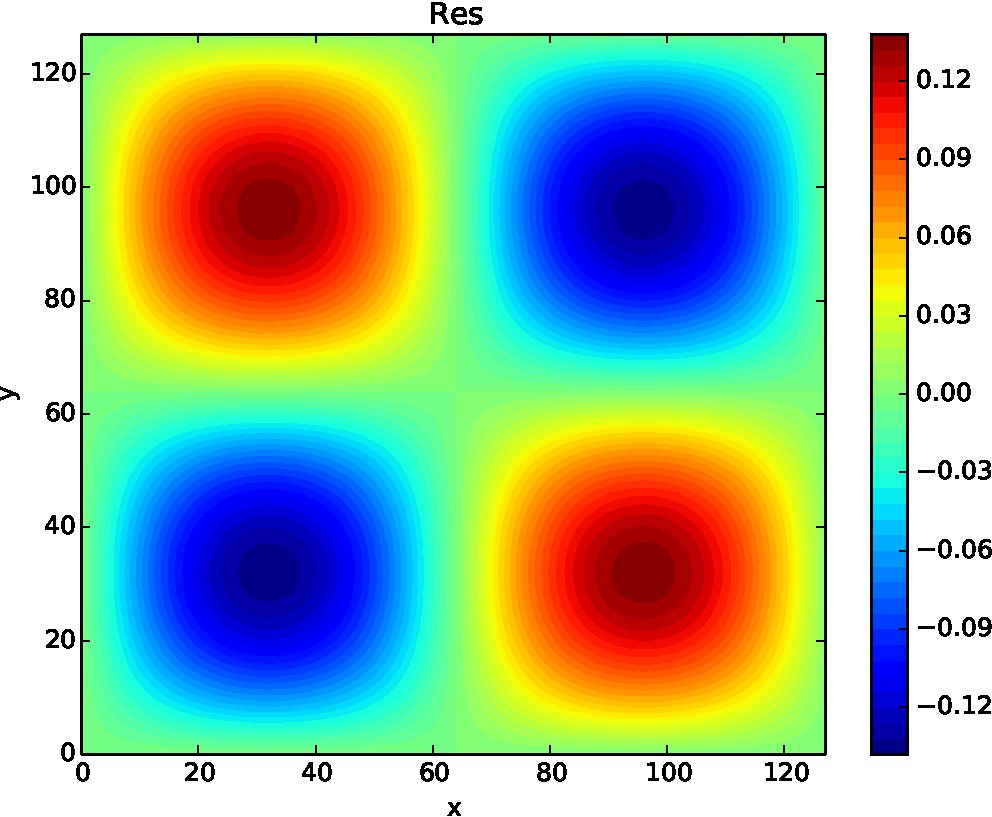
\includegraphics[width = \textwidth]{figures/verification/sinusoidal/residual.pdf}
	% 			% \end{subfigure}
	% 		\caption{This a \(x,y\)-plane from the grids cut along \(z_l = 32\), from the sinusoidal test case described in \cref{sec:sinusoidal}.
	% 		The left plot shows the charge distribution, the center plot shows the numerical solution of the potential and the plot to the right depicts
	% 		the residual.}
	% 		\label{fig:sinusoidal}
	% 	\end{figure}
	%
	% 	The \cref{fig:sinusoidal} shows the results from running the MG-solver on the test sinusoidal test case described here.
	% 	As can be expected the potential mirrors the charge distribution, except with an opposite sign and a larger amplitude.
	% 	A decently large grid was simulated and the mean residual was found to be: \(\bar{r} \approx 0.0312\).
	%
	%
	% 	\subsubsection{Heaviside Function}
	% 		The solver is also tested with a charge distribution governed by a Heaviside
	% 		function. This is also suited to testing since the charge distribution is then
	% 		constant planes, and we expect second order polynomial when integrating them.
	% 		In the test case there are two planes with the value \(-1\) and two
	% 		planes with \(1\). In \cref{fig:heaviside} the test case, as well as the solution and residual is
	% 		shown, and we can see the polynomials in the solution. The mean residual \(\bar{r}\) was
	% 		\(0.00677\).
	%
	% 	\begin{align}
	% 		\rho_(x_j,y_k,z_l) &= \begin{cases} 1  & y_j \epsilon (0, 32), (64,96)\\ -1  & y_j \epsilon (33, 65), (97,127) \end{cases}
	% 	\end{align}
	%
	% 	\begin{figure}
	% 		\centering
	% 			% \begin{subfigure}[b]{0.32\textwidth}
	% 			% 	\includegraphics[width = \textwidth]{figures/verification/heaviside/rho.pdf}
	% 			% \end{subfigure}
	% 			% \begin{subfigure}[b]{0.32\textwidth}
	% 			% 	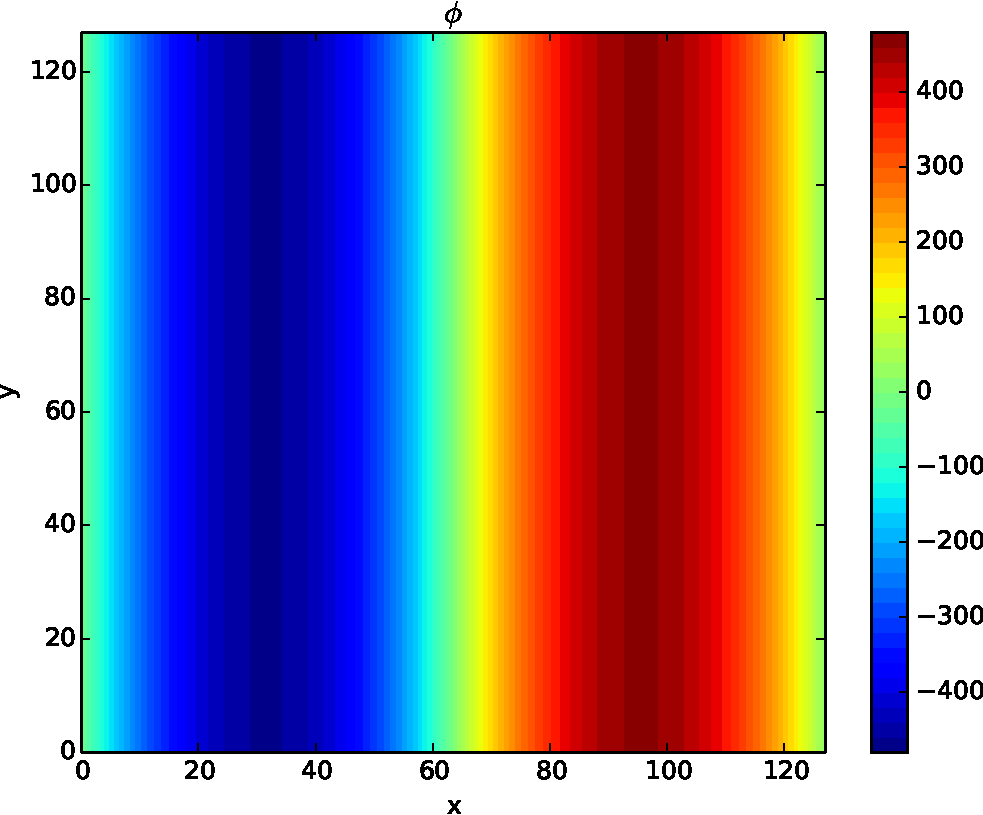
\includegraphics[width = \textwidth]{figures/verification/heaviside/phi.pdf}
	% 			% \end{subfigure}
	% 			% \begin{subfigure}[b]{0.32\textwidth}
	% 			% 	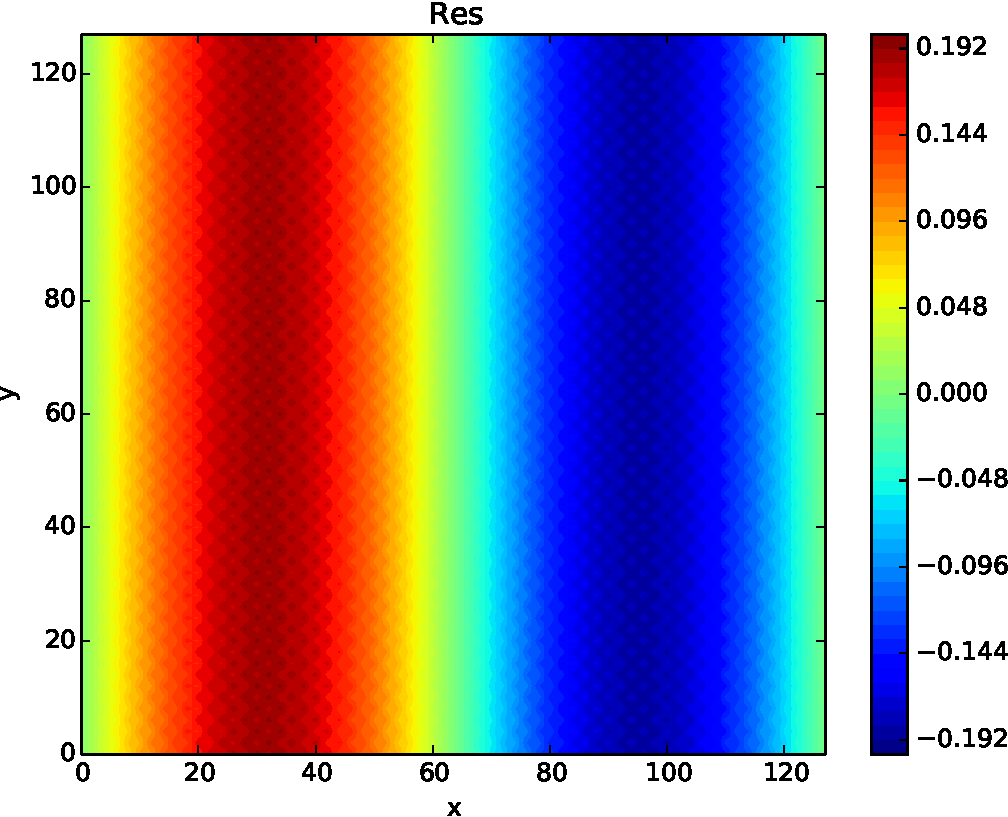
\includegraphics[width = \textwidth]{figures/verification/heaviside/residual.pdf}
	% 			% \end{subfigure}
	% 		\caption{As earlier this is a \(x,y\)-plane cut along \(x_k=32\), of the grid. The plots show the charge distribution,
	% 		numerical solution and the solution, from left to right. This is a test case constructed
	% 		with Heaviside functions. In the solution of the potential the expected second degree polynomial can be seen.
	% 		}
	% 		\label{fig:heaviside}
	% 	\end{figure}
	%
	% 	\subsection{Random Charge distribution}
	% 		To hopefully avoid some problems, that could appear due to the earlier test
	% 		cases being to constructed being to orderly, a test with a randomized
	% 		charge distribution is also included. The \cref{fig:random} shows the
	% 		charge distribution, numerical potential and the residual. The mean residual was
 % 			found to be \(\bar{r} \approx 0.00388\).
	% 		%
	% 		\begin{figure}
	% 			\centering
	% 			% \begin{subfigure}[b]{0.32\textwidth}
	% 			% 	\includegraphics[width = \textwidth]{figures/verification/random/rho.pdf}
	% 			% \end{subfigure}
	% 			% \begin{subfigure}[b]{0.32\textwidth}
	% 			% 	\includegraphics[width = \textwidth]{figures/verification/random/phi.pdf}
	% 			% \end{subfigure}
	% 			% \begin{subfigure}[b]{0.32\textwidth}
	% 			% 	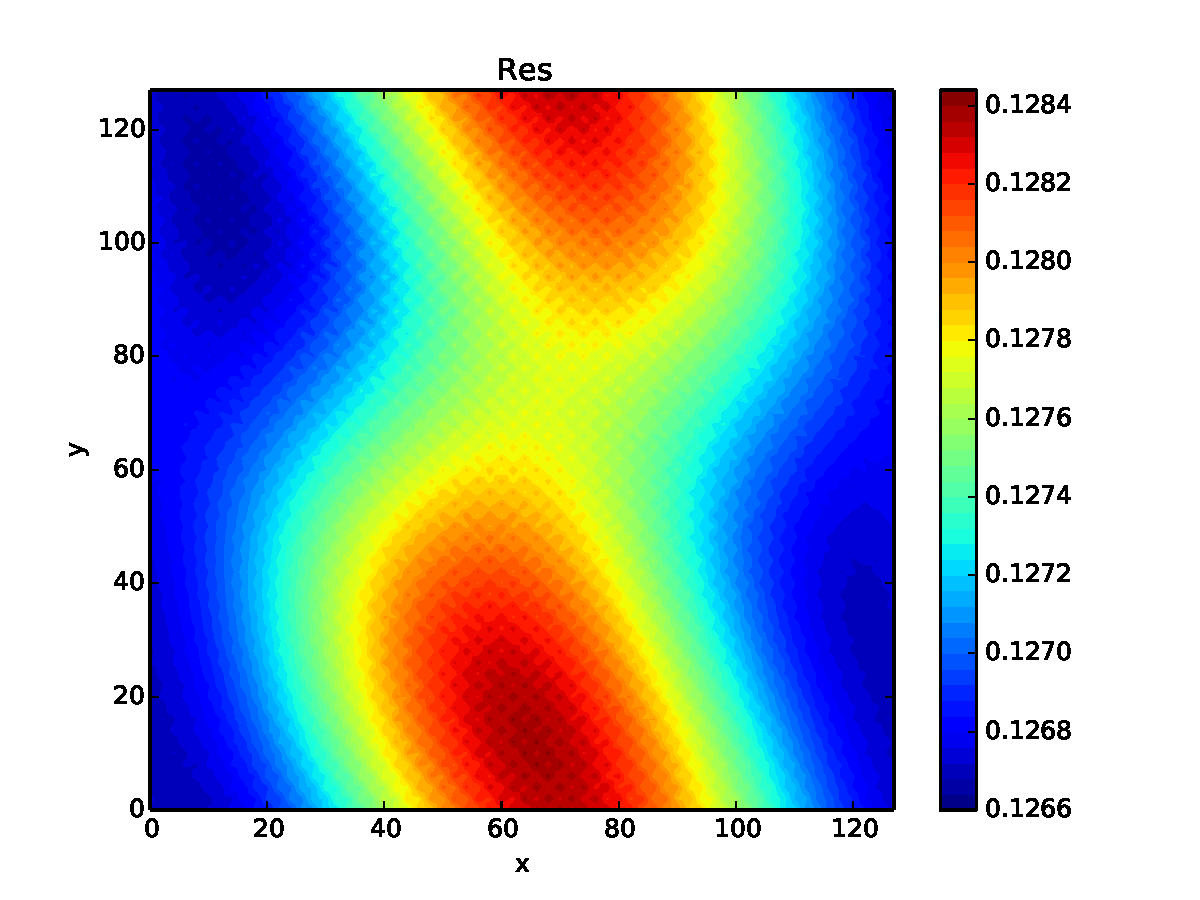
\includegraphics[width = \textwidth]{figures/verification/random/residual.pdf}
	% 			% \end{subfigure}
	% 			\caption{As earlier this is a \(x,y\)-plane cut along \(x_k=32\), of the grid. The plots show the charge distribution,
	% 			numerical solution and the solution, from left to right.}
	% 			\label{fig:random}
	% 		\end{figure}
%
% \section{Multigrid Solver}
% 	To test the solver itself we employ a couple different techniques. First we
% 	create a charge distribution by differentiating a known potential, and then
% 	running the solver and check if the resulting potential was equal to the original
% 	known potential.
%
% 	For the second test we use a charge distribution with a known analytical solution,
% 	and we then check that the solver reproduces the known analytical solution.
%
% 	A third method we use to verify it is to produce a random charge potential
% 	and then check that the potential converges, or in other words
% 	that the residual goes toward zero.
%
% 	Then lastly we use the solver on identical charge distributions with the domain
% 	divided up into different subdomains and check that the solver produces the same
% 	potential.
% \subsection{Predetermined Potential}
% 		In this section we first decide which potential we want, then numerically
% 		construct a corresponding charge potential by derivating. Then we compare the
% 		result with the original potential.

		% In
		%
		% \begin{figure}
		% 	\centering
		% 		\begin{subfigure}
		% 	% 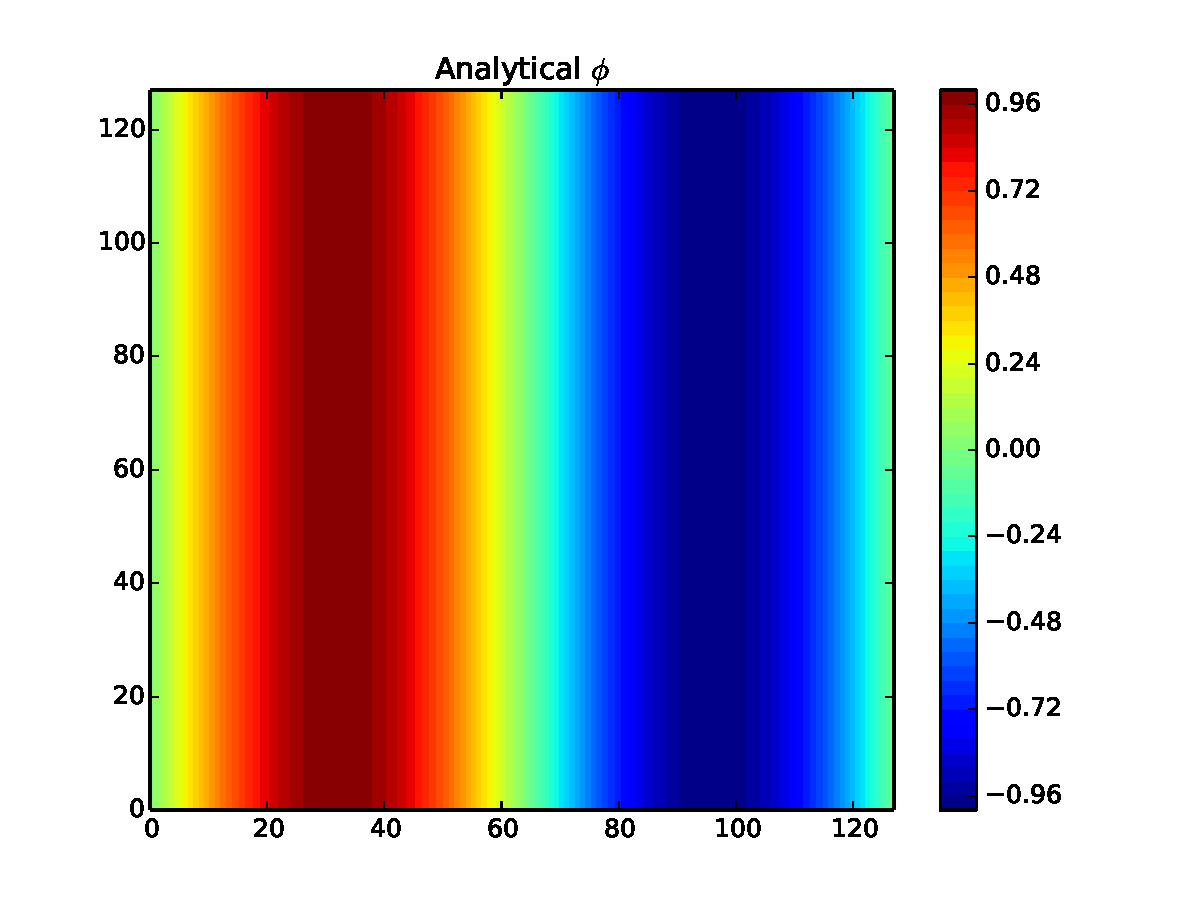
\includegraphics[width = 0.45\textwidth]{figures/verification/sinusoidal/analytical.pdf}
		% 	\end{subfigure}
		% 		\begin{subfigure}
		% 	% 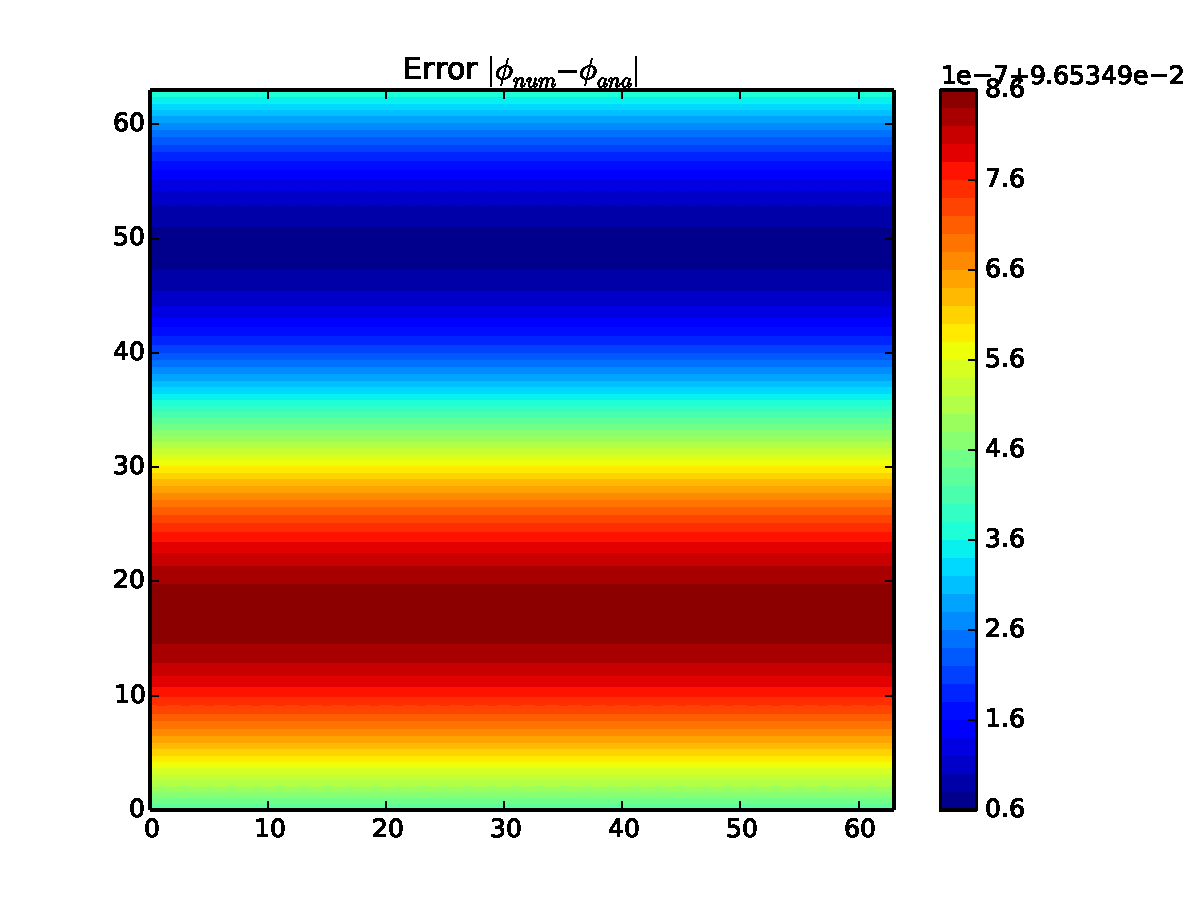
\includegraphics[width = 0.45\textwidth]{figures/verification/sinusoidal/error.pdf}
		% \end{subfigure}
		% \end{figure}
		%

		\subsection{Convergence of Residual}
		(TBD)

		\subsection{Different Domain divisions}
		(TBD)

% \section{Particle-in-Cell}
%
% 	\subsection{Plasma Oscillations}
%
% \textbf{NB! See if something below is salvageable}
%
%
% The multigrid method has several different steps in the algorithm, as a developmental
% help and to ensure that the program works correctly during as many different conditions
% as possible we want to test the whole code, as well as the constituent parts where possible.
% The method is quite modular and several parts of it can be tested alone.
% The GS-RB, used for smoothing, can be independently tested, since on it's own it converges to a solution,
% just at a higher computational cost than the multigrid method. To test it we will
% use an initial density field with a length between the grid steps that results in
% an exact answer. The restriction and prolongation operators can also tested to a
% degree by checking that they preserve a constant grid through several grid level changes.
%
%
% The multigrid method has several different steps in the algorithm, as a developmental
% help and to ensure that the program works correctly during as many different conditions
% as possible we want to test the whole code, as well as the constituent parts where possible.
% The method is quite modular and several parts of it can be tested alone.
% The GS-RB, used for smoothing, can be independently tested, since on it's own it converges to a solution,
% just at a higher computational cost than the multigrid method. To test it we will
% use an initial density field with a length between the grid steps that results in
% an exact answer. The restriction and prolongation operators can also tested to a
% degree by checking that they preserve a constant grid through several grid level changes.
%
% \subsection{The Multigrid method}
% 	We use both of the aforemented tests to check that the whole multigrid method
% 	works as intended. Since a constant source term will give a trivial solution of
% 	the potential, \(\phi(x,y,z) = \va{0}\), we use that as a test. In addition we
% 	also test that it converges on a sinusoidal source term as we did the smoother.
%
%
% \subsection{Smoothers}
%
% 	The iterative method GS-RB used for the pre- and postsmoothing of the grid in
% 	our implementation of the multigrid method is also a direct solver.
% 	So we can test it, or most other smoothers, by testing them on a small system
% 	where the problem has an analytical solution. Then we can let them run for a
% 	while and ensure that they are converging towards the solution. If we let
% 	the source term be sinusoidal in one direction, and constant in the other
% 	directions it has an easy solution given below
%
% 	\begin{align}
% 		\nabla^2 \phi(x,y,z) &= \sin(x)
% 	\end{align}
%
% 	This has a solution when \(\phi(x,y,z) = -\sin(x)\) and we can test that the
% 	solver converges to the solution. If we let the source term be constant in the
% 	x direction and instead vary in the other directions we can get verify that the
% 	solver works in all three directions independently.



\printbibliography

\end{document}


